
\documentclass[12pt,journal]{IEEEtran}
% The Computer Society requires 12pt.
% If IEEEtran.cls has not been installed into the LaTeX system files,
% manually specify the path to it like:
% \documentclass[10pt,journal,compsoc]{../sty/IEEEtran}

% For Computer Society journals, IEEEtran defaults to the use of 
% Palatino/Palladio as is done in IEEE Computer Society journals.
% To go back to Times Roman, you can use this code:
%\renewcommand{\rmdefault}{ptm}\selectfont

% Some very useful LaTeX packages include:

\usepackage[utf8]{inputenc}
\usepackage{listings}
\usepackage{xcolor}
\usepackage{graphicx}

\ifCLASSOPTIONcompsoc
  \usepackage[caption=false,font=normalsize,labelfont=sf,textfont=sf]{subfig}
\else
  \usepackage[caption=false,font=footnotesize]{subfig}
\fi
% subfig.sty, written by Steven Douglas Cochran, is the modern replacement
% for subfigure.sty, the latter of which is no longer maintained and is
% incompatible with some LaTeX packages including fixltx2e. However,
% subfig.sty requires and automatically loads Axel Sommerfeldt's caption.sty
% which will override IEEEtran.cls' handling of captions and this will result
% in non-IEEE style figure/table captions. To prevent this problem, be sure
% and invoke subfig.sty's "caption=false" package option (available since
% subfig.sty version 1.3, 2005/06/28) as this is will preserve IEEEtran.cls
% handling of captions.
% Note that the Computer Society format requires a larger sans serif font
% than the serif footnote size font used in traditional IEEE formatting
% and thus the need to invoke different subfig.sty package options depending
% on whether compsoc mode has been enabled.
%
% The latest version and documentation of subfig.sty can be obtained at:
% http://www.ctan.org/tex-archive/macros/latex/contrib/subfig/


\definecolor{mygreen}{rgb}{0,0.6,0}
\definecolor{mygray}{rgb}{0.5,0.5,0.5}
\definecolor{mymauve}{rgb}{0.58,0,0.82}

\lstset{ %
  backgroundcolor=\color{white},   % choose the background color; you must add \usepackage{color} or \usepackage{xcolor}
  basicstyle=\footnotesize,        % the size of the fonts that are used for the code
  breakatwhitespace=false,         % sets if automatic breaks should only happen at whitespace
  breaklines=true,                 % sets automatic line breaking
  captionpos=n,                    % sets the caption-position
  commentstyle=\color{mygreen},    % comment style
  deletekeywords={...},            % if you want to delete keywords from the given language
  escapeinside={\%*}{*)},          % if you want to add LaTeX within your code
  extendedchars=true,              % lets you use non-ASCII characters; for 8-bits encodings only, does not work with UTF-8
  frame=single,                    % adds a frame around the code
  keepspaces=true,                 % keeps spaces in text, useful for keeping indentation of code (possibly needs columns=flexible)
  keywordstyle=\color{blue},       % keyword style
  language=C,                 		% the language of the code
  morekeywords={"visit_handle"},            % if you want to add more keywords to the set
  numbers=left,                    % where to put the line-numbers; possible values are (none, left, right)
  numbersep=5pt,                   % how far the line-numbers are from the code
  numberstyle=\tiny\color{mygray}, % the style that is used for the line-numbers
  rulecolor=\color{black},         % if not set, the frame-color may be changed on line-breaks within not-black text (e.g. comments (green here))
  showspaces=false,                % show spaces everywhere adding particular underscores; it overrides 'showstringspaces'
  showstringspaces=false,          % underline spaces within strings only
  showtabs=false,                  % show tabs within strings adding particular underscores
  stepnumber=2,                    % the step between two line-numbers. If it's 1, each line will be numbered
  stringstyle=\color{mymauve},     % string literal style
  tabsize=2,                       % sets default tabsize to 2 spaces
  title=\lstname                   % show the filename of files included with \lstinputlisting; also try caption instead of title
}


% *** Do not adjust lengths that control margins, column widths, etc. ***
% *** Do not use packages that alter fonts (such as pslatex).         ***
% There should be no need to do such things with IEEEtran.cls V1.6 and later.
% (Unless specifically asked to do so by the journal or conference you plan
% to submit to, of course. )


% correct bad hyphenation here
\hyphenation{op-tical net-works semi-conduc-tor}


\begin{document}

%
% paper title
% can use linebreaks \\ within to get better formatting as desired
% Do not put math or special symbols in the title.
\title{SmartBierdeggl}
%
%
% author names and IEEE memberships
% note positions of commas and nonbreaking spaces ( ~ ) LaTeX will not break
% a structure at a ~ so this keeps an author's name from being broken across
% two lines.
% use \thanks{} to gain access to the first footnote area
% a separate \thanks must be used for each paragraph as LaTeX2e's \thanks
% was not built to handle multiple paragraphs

\author{Achim~Herrmann,
        Achim~Däubler}

% The paper headers
\markboth{SmartBierdeggl Dokumentation, Februar~2016}%
{%Shell \MakeLowercase{\textit{et al.}}: Bare Advanced Demo of IEEEtran.cls for Journals}
}
% The only time the second header will appear is for the odd numbered pages
% after the title page when using the twoside option.
% 
% *** Note that you probably will NOT want to include the author's ***
% *** name in the headers of peer review papers.                   ***
% You can use \ifCLASSOPTIONpeerreview for conditional compilation here if
% you desire.

% make the title area
\maketitle

% for Computer Society papers, we must declare the abstract and index terms
% PRIOR to the title within the \IEEEtitleabstractindextext IEEEtran
% command as these need to go into the title area created by \maketitle.
% As a general rule, do not put math, special symbols or citations
% in the abstract or keywords.
%\IEEEtitleabstractindextext{%
\begin{abstract}
Ziel des Projektes SmartBierdeggl ist es einen Bierdeckel zu konstruieren, der automatisch mitzählt wieviele Getränke man bereits hat.\\
Er besteht aus einer Wägezelle, mit der das Gewicht des darauf abgestellten Getränks gemessen wird.
Außerdem enthält er einen Mikrocontroller, der die gemessenen Gewichtsdaten erhält und daraus errechnet ob ein neues Getränk abgestellt wurde oder nicht.
Wie viele neue Getränke schon abgestellt wurden wird durch LEDs am Bierdeckel veranschaulicht.
\end{abstract}
%}

\section{Einleitung}

% The very first letter is a 2 line initial drop letter followed
% by the rest of the first word in caps (small caps for compsoc).
% 
% form to use if the first word consists of a single letter:
% \IEEEPARstart{A}{demo} file is ....
% 
% form to use if you need the single drop letter followed by
% normal text (unknown if ever used by IEEE):
% \IEEEPARstart{A}{}demo file is ....
% 
% Some journals put the first two words in caps:
% \IEEEPARstart{T}{his demo} file is ....
% 
% Here we have the typical use of a "T" for an initial drop letter
% and "HIS" in caps to complete the first word.
\IEEEPARstart{Z}{uerst} wird der Aufbau des Bierdeckels beschrieben.
Es wird erklärt, welche Bestandteile benötigt werden und wie sie funktionieren.
Dann zeigen wir unser Platinendesign, das die Bauteile miteinander verbindet.
Zum Schluss wird anhand unseres Codes veranschaulicht, wie die Gewichtsmessung funktioniert.

\section{Vorabüberlegungen}
Zunächst wird eine Möglichkeit benötigt, welche die automatische Detektion eines neuen Getränks ermöglicht.
Hierfür fiel die Wahl auf Überwachung des aktuellen Gewichts auf dem Bierdeckel.
Die Grundlage für die Gewichtsmessung sind Dehnmessstreifen (DMS).
Diese ändern bei Dehnung bzw. Stauchung ihren elektrischen Widerstand.
Zusammen mit weiteren DMS oder Widerständen kann man damit eine sogenannte Wheatstonesche Messbrücke (Abb. \ref{fig_wheatstone}) konstruieren.
\begin{figure}[!h]
  \centering
    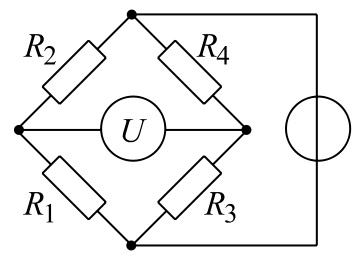
\includegraphics[width=3.6in]{images/wheatstone.png}
    \caption{Wheatstone'sche Brücke}
  \label{fig_wheatstone}
\end{figure}
Ersetzt man in Abb. \ref{fig_wheatstone} nun einen oder mehrere Widerstände durch DMS, so führen Dehnungen oder Stauchungen auf diesen zu Spannungsänderungen.
Befestigt man nun die DMS an einem geeigneten Federkörper so erhält man eine sog. Wägezelle (engl. Load Cell, Abb. \ref{fig_loadcell}), welche für das Projekt verwendet wurden.
\begin{figure}[!h]
  \centering
    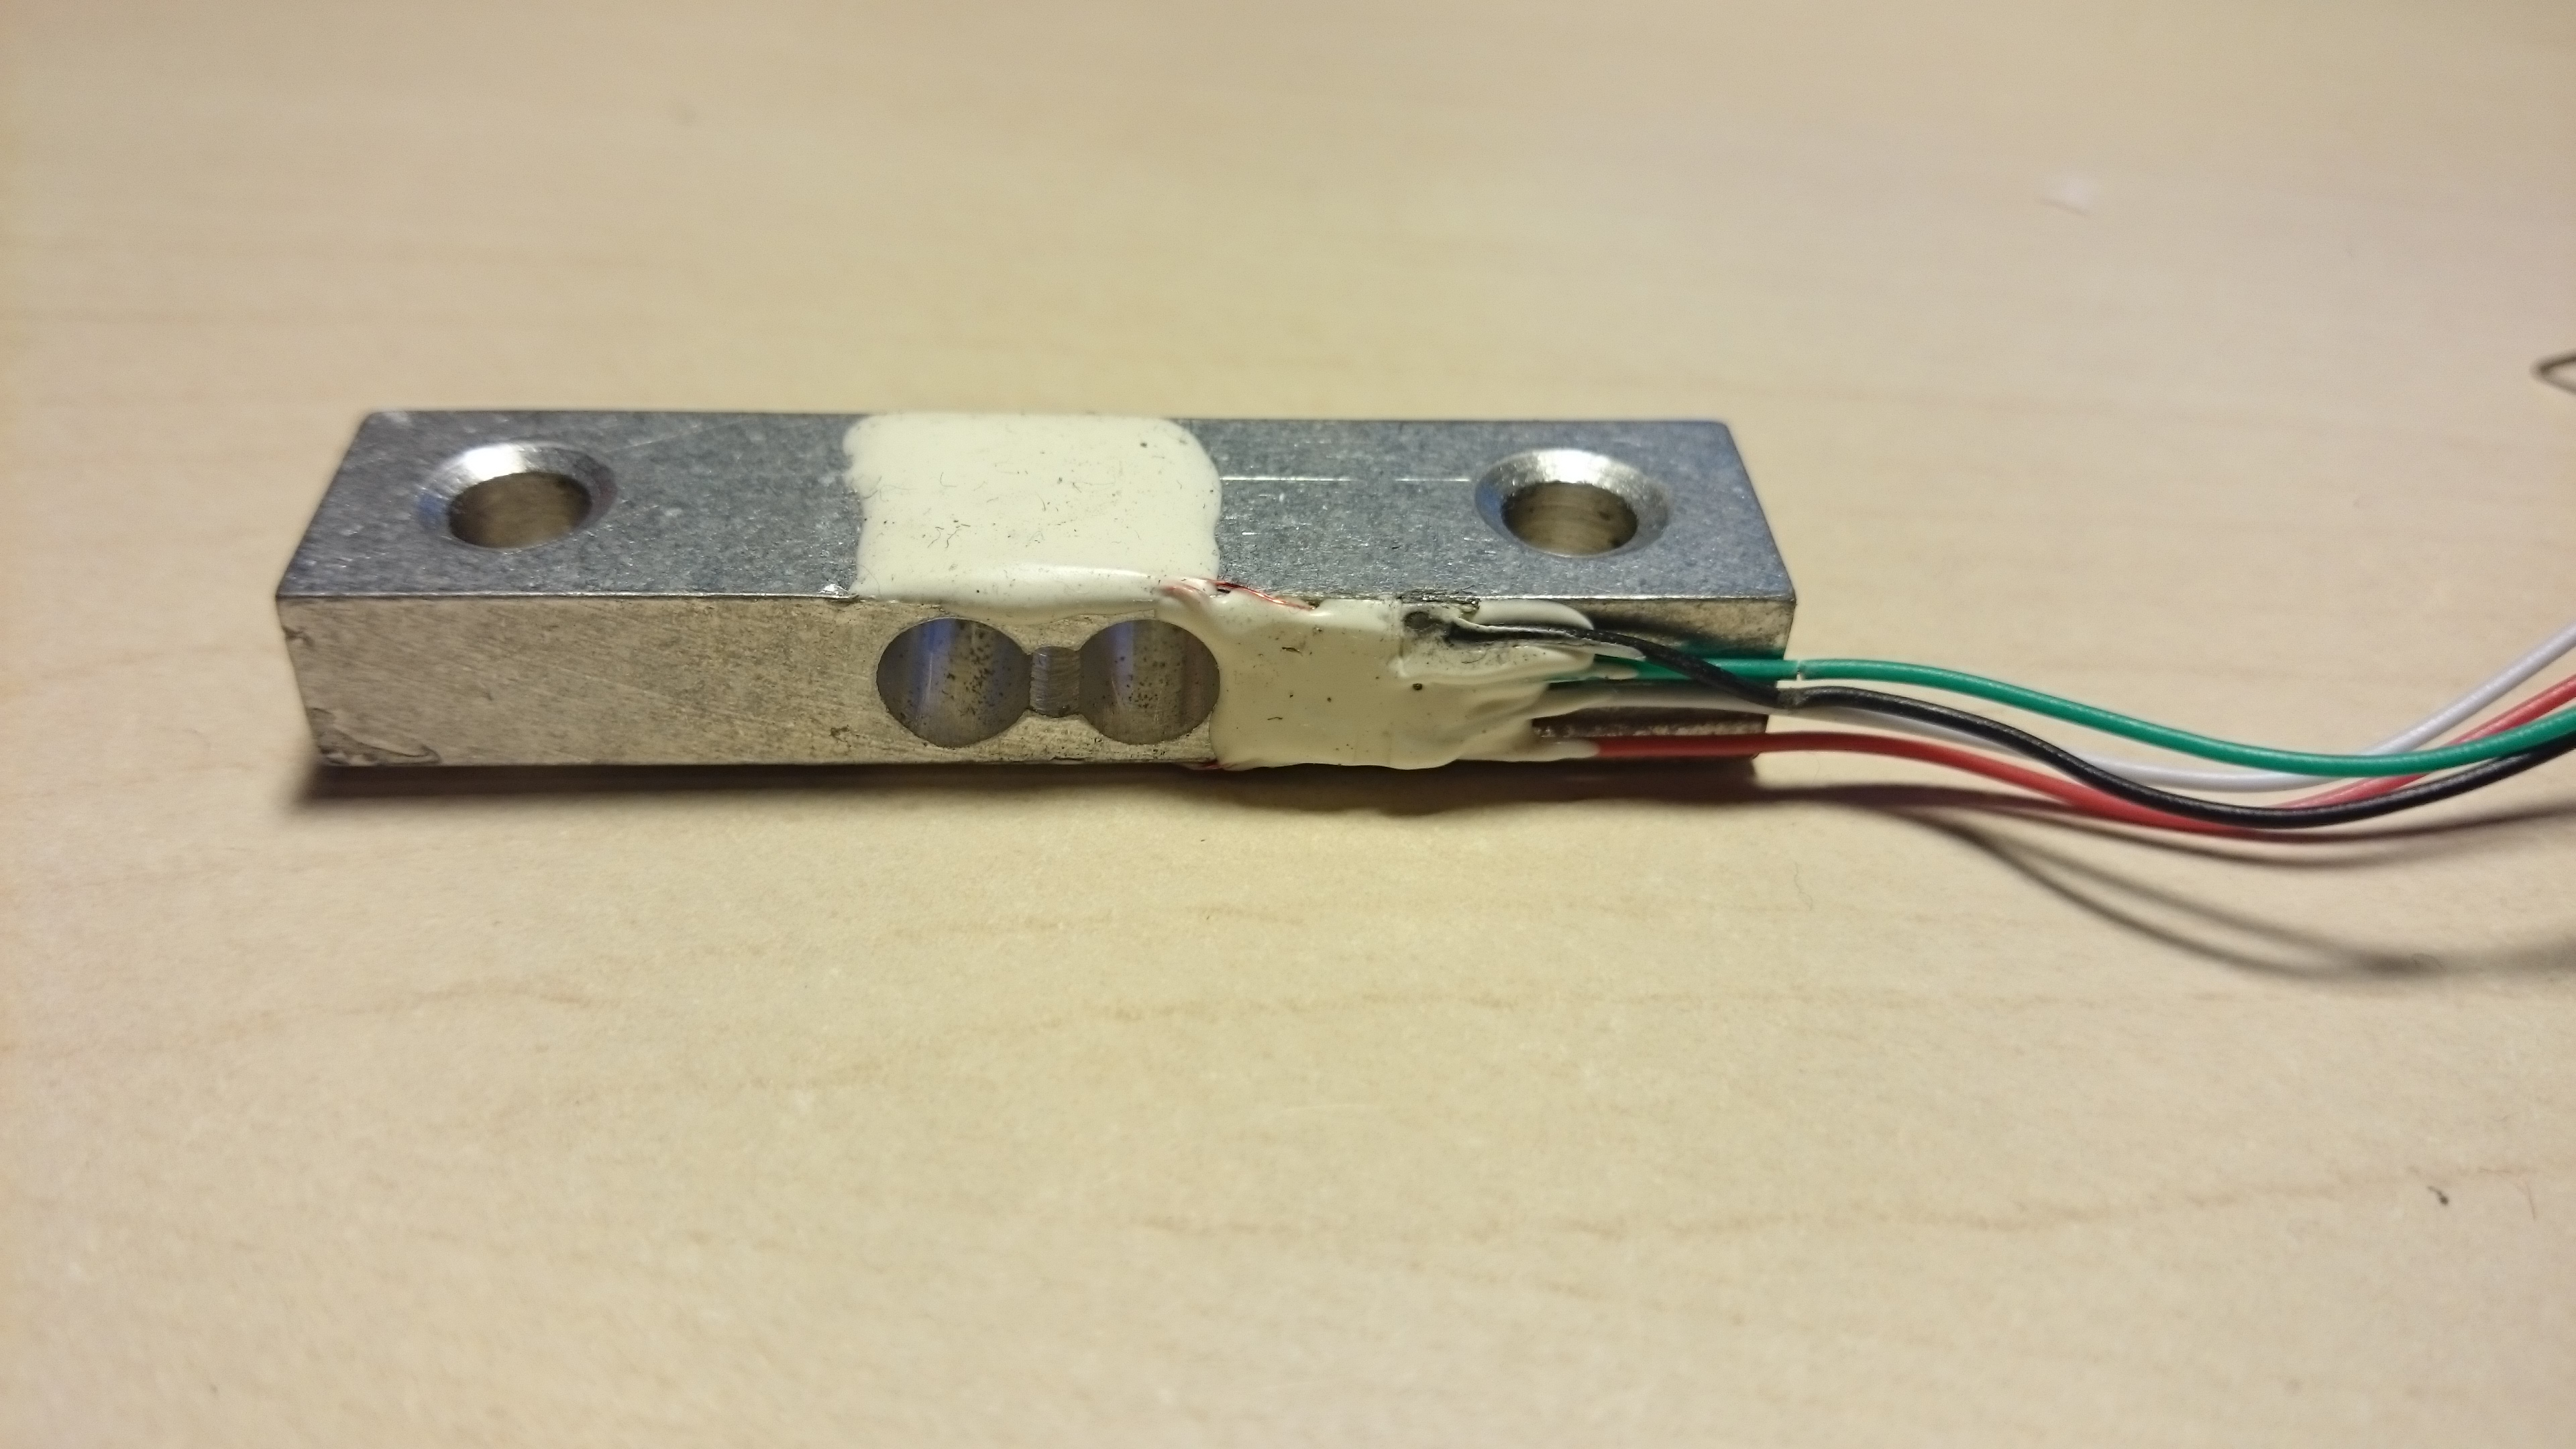
\includegraphics[width=3.5in]{images/loadcell.jpg}
    \caption{Wägezelle}
  \label{fig_loadcell}
\end{figure}
Es ist auch möglich die Messstreifen direkt an dem Bierdeckel zu befestigen, dies wurde allerdings aufgrund der hohen Kosten für einen DMS im Vergleich zu einer Wägezelle verworfen.
Um die Daten der Wägezelle in einem Microcontroller verarbeiten zu können, benötigt man einen Analog-Digital Wandler.
Dieser kann bereits in dem Mircocontoller vorhanden sein.
In diesem Fall wird jedoch noch ein Signalverstärker benötigt.
Eine andere Möglichkeit ist die Verwendung eines dedizierten Moduls, wie dem HX711 \cite{hx711sheet} (Abb. \ref{fig_HX711_board}).
\begin{figure}[h]
  \centering
    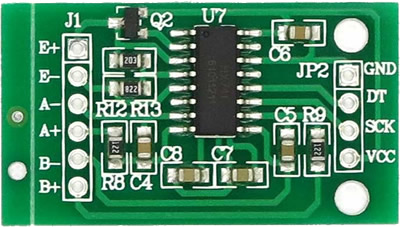
\includegraphics[width=3.5in]{images/HX711Board.jpeg}
    \caption{HX711 Board}
  \label{fig_HX711_board}
\end{figure}
Dieser wandelt das analoge Signal der Wägezelle in einen 24 bit Digitalwert, welcher durch den Microcontroller ausgelesen werden kann.
\begin{figure*}[htbp]
\centering
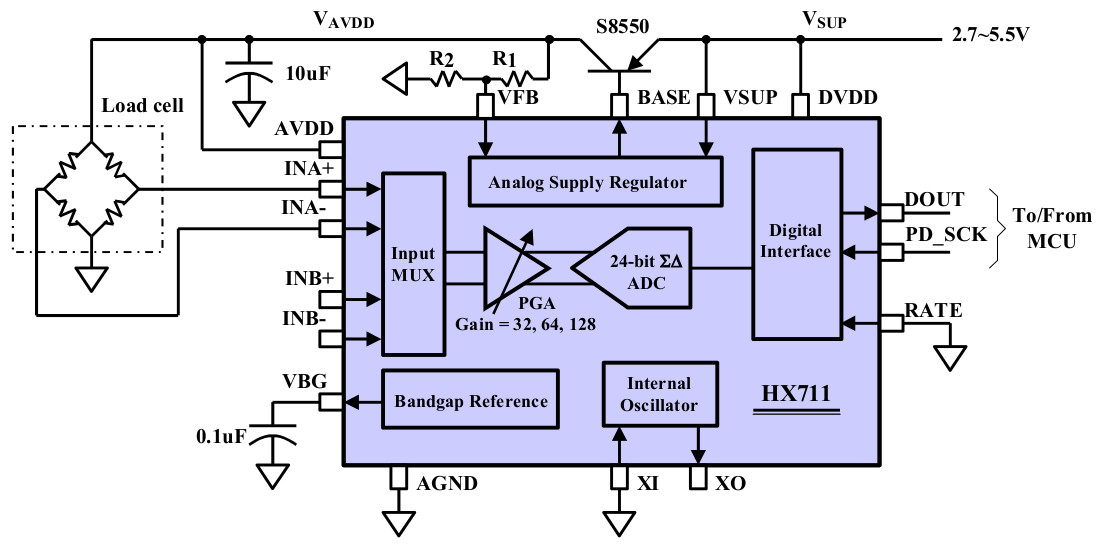
\includegraphics[width=7in]{images/HX711.jpg}%
\caption{HX711 Beschaltung}
\label{fig_HX711}
\end{figure*}

\pagebreak

\section{Funktionsweise des HX711}


Der Aufbau der Platine, die den  HX711 IC enthält, ist in Fig. \ref{fig_HX711} dargestellt.
Wie man in der Abbildung sehen kann werden die Pins AVDD, AGND, INA+ und INA- und  (entspricht
E+, E-, A+ und A- auf der Platine in Abbildung \ref{fig_HX711_board}) des HX711 mit
der Wägezelle verbunden. Jetzt wird gemäß der Wheatstone Brückenschaltung die Spannungsdifferenz
zwischen INA+ und INA- gemessen. Dann wird sie verstärkt und vom 24 Bit Analog-zu-Digitalkonverter
und in einen Digitalwert umgewandelt. Dieser muss nun ausgelesen werden.\\
Die Pins PD\_SCK und DOUT (entspricht SCK und DT in Fig. \ref{fig_HX711_board}) werden für den Datenaustausch
verwendet. Sobald DOUT von HIGH auf LOW wechselt, sind Daten zur Abholung bereit.
Dann müssen 25 positive Taktsignale an PD\_SCK geschickt werden (PD\_SCK muss mindestens 2$\mu$s lang
HIGH und 2$\mu$s LOW sein, also nicht zu schnell lesen!), wobei jedes ein Bit aus DOUT shifted.
Begonnen wird dabei mit dem MSB Bit. Der 25. Takt zieht DOUT wieder auf HIGH.
Indem weitere Takte gesendet werden (höchstens 27) kann man für das nächste Signal wählen
ob Eingang A oder B ausgelesen wird welchen Gain das gelesene Signal bekommen soll. 

PD\_SCK wird außerdem verwendet um den HX711 resetten. Wenn der Pin länger als 60$\mu$s auf HIGH
steht dann wird der Power Down Mode aktiviert. Wenn der Pin wieder auf LOW gezogen wird,
dann setzt sich der Chip zurück und geht in den normalen Betriebsmodus über.

\section{Aufbau}

\noindent
Der SmartBierdeggl besteht aus folgenden Teilen:
\begin{itemize}
\item Microcontroller
\item Wägezelle
\item HX711
\item LEDs
\item Stromversorgung
\end{itemize}
Die Wägezelle stammte hierbei von einer Küchenwaage, welche sich auch gut zum Testen eignete.
Als Microcontroller wurde anfangs das TinyUSBBoard \cite{tinyusb} verwendet.
Dies wurde für Testzwecke, auf Grundlage des EasyLogger \cite{easylogger}, um eine USB-Ausgabe Funktionalität erweitert.
Jedoch stellte sich heraus, dass die USB-Ausgabe mit dem Timing des HX711 interferiert.
Infolge dessen wurde statt des TinyUSBBoard  ein UNO-Board verwendet, welches das Testen über eine serielle Schnittstelle ermöglicht.
Sobald das System lief, wurde auf einen separaten Mircocontroller umgestiegen.
Dies ist aktuell noch ein Atmel ATMega328PA, dieser kann jedoch ohne weiteres durch einen ATMega48 ersetzt werden.
Um diesen herum wurde anschließend auf einem Steckboard ein Prototyp für den SmartBierdeggl entworfen (Abb. \ref{fig_prototyp}).
Als Stromversorgung dienen hierbei 3 AA Batterien mit jeweils 1,5V.
\begin{figure*}[!t]
\centering
\subfloat[Atmega328p Pin Belegung]{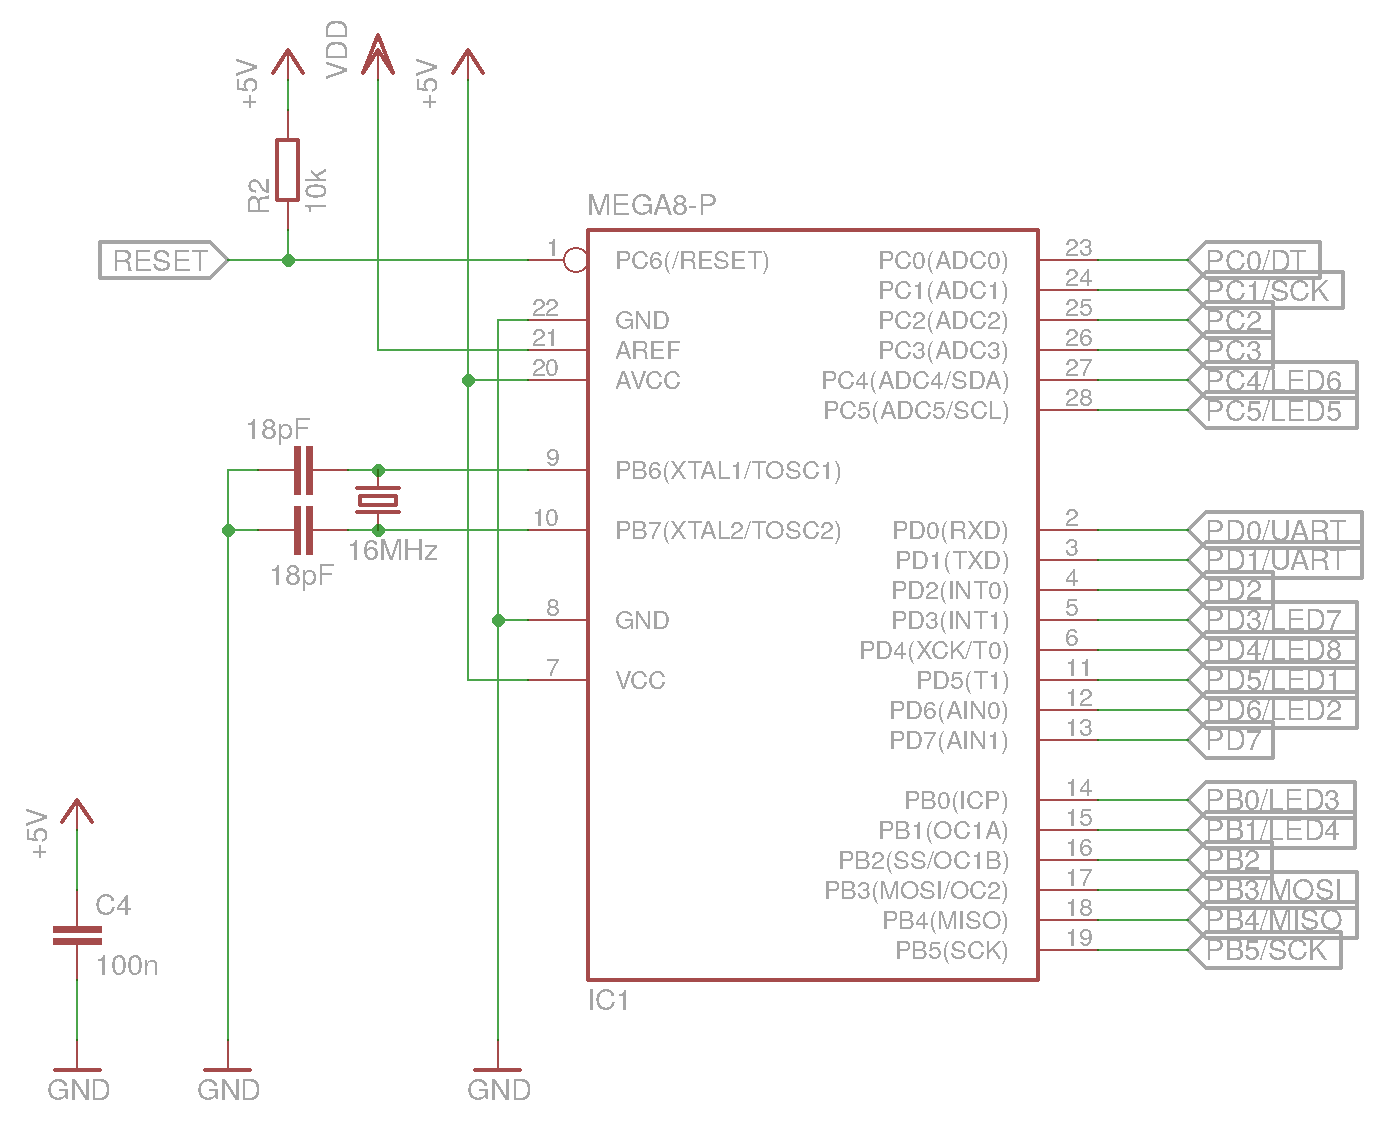
\includegraphics[width=4.3in]{images/atmega328p_pin_belegung.png}%
\label{fig_atmega328_pin}}
\hfil
\subfloat[Konnektoren]{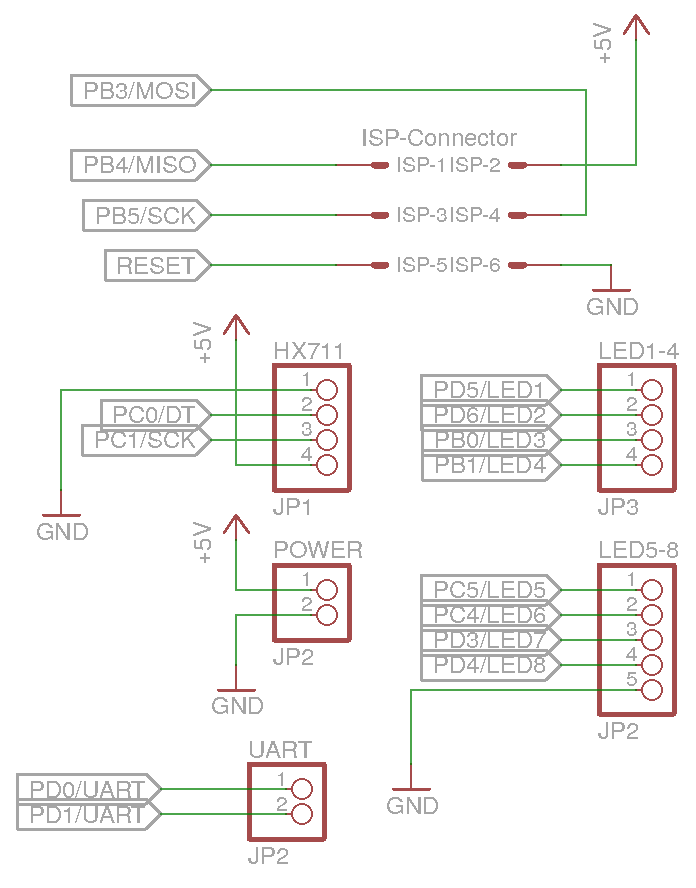
\includegraphics[width=2.8in]{images/bierdeckel_board_connectors.png}%
\label{fig_board_connectors}}
\caption{Beschaltung des Atmega328p}
\label{fig_sim}
\end{figure*}

\begin{figure}[h]
  \centering
    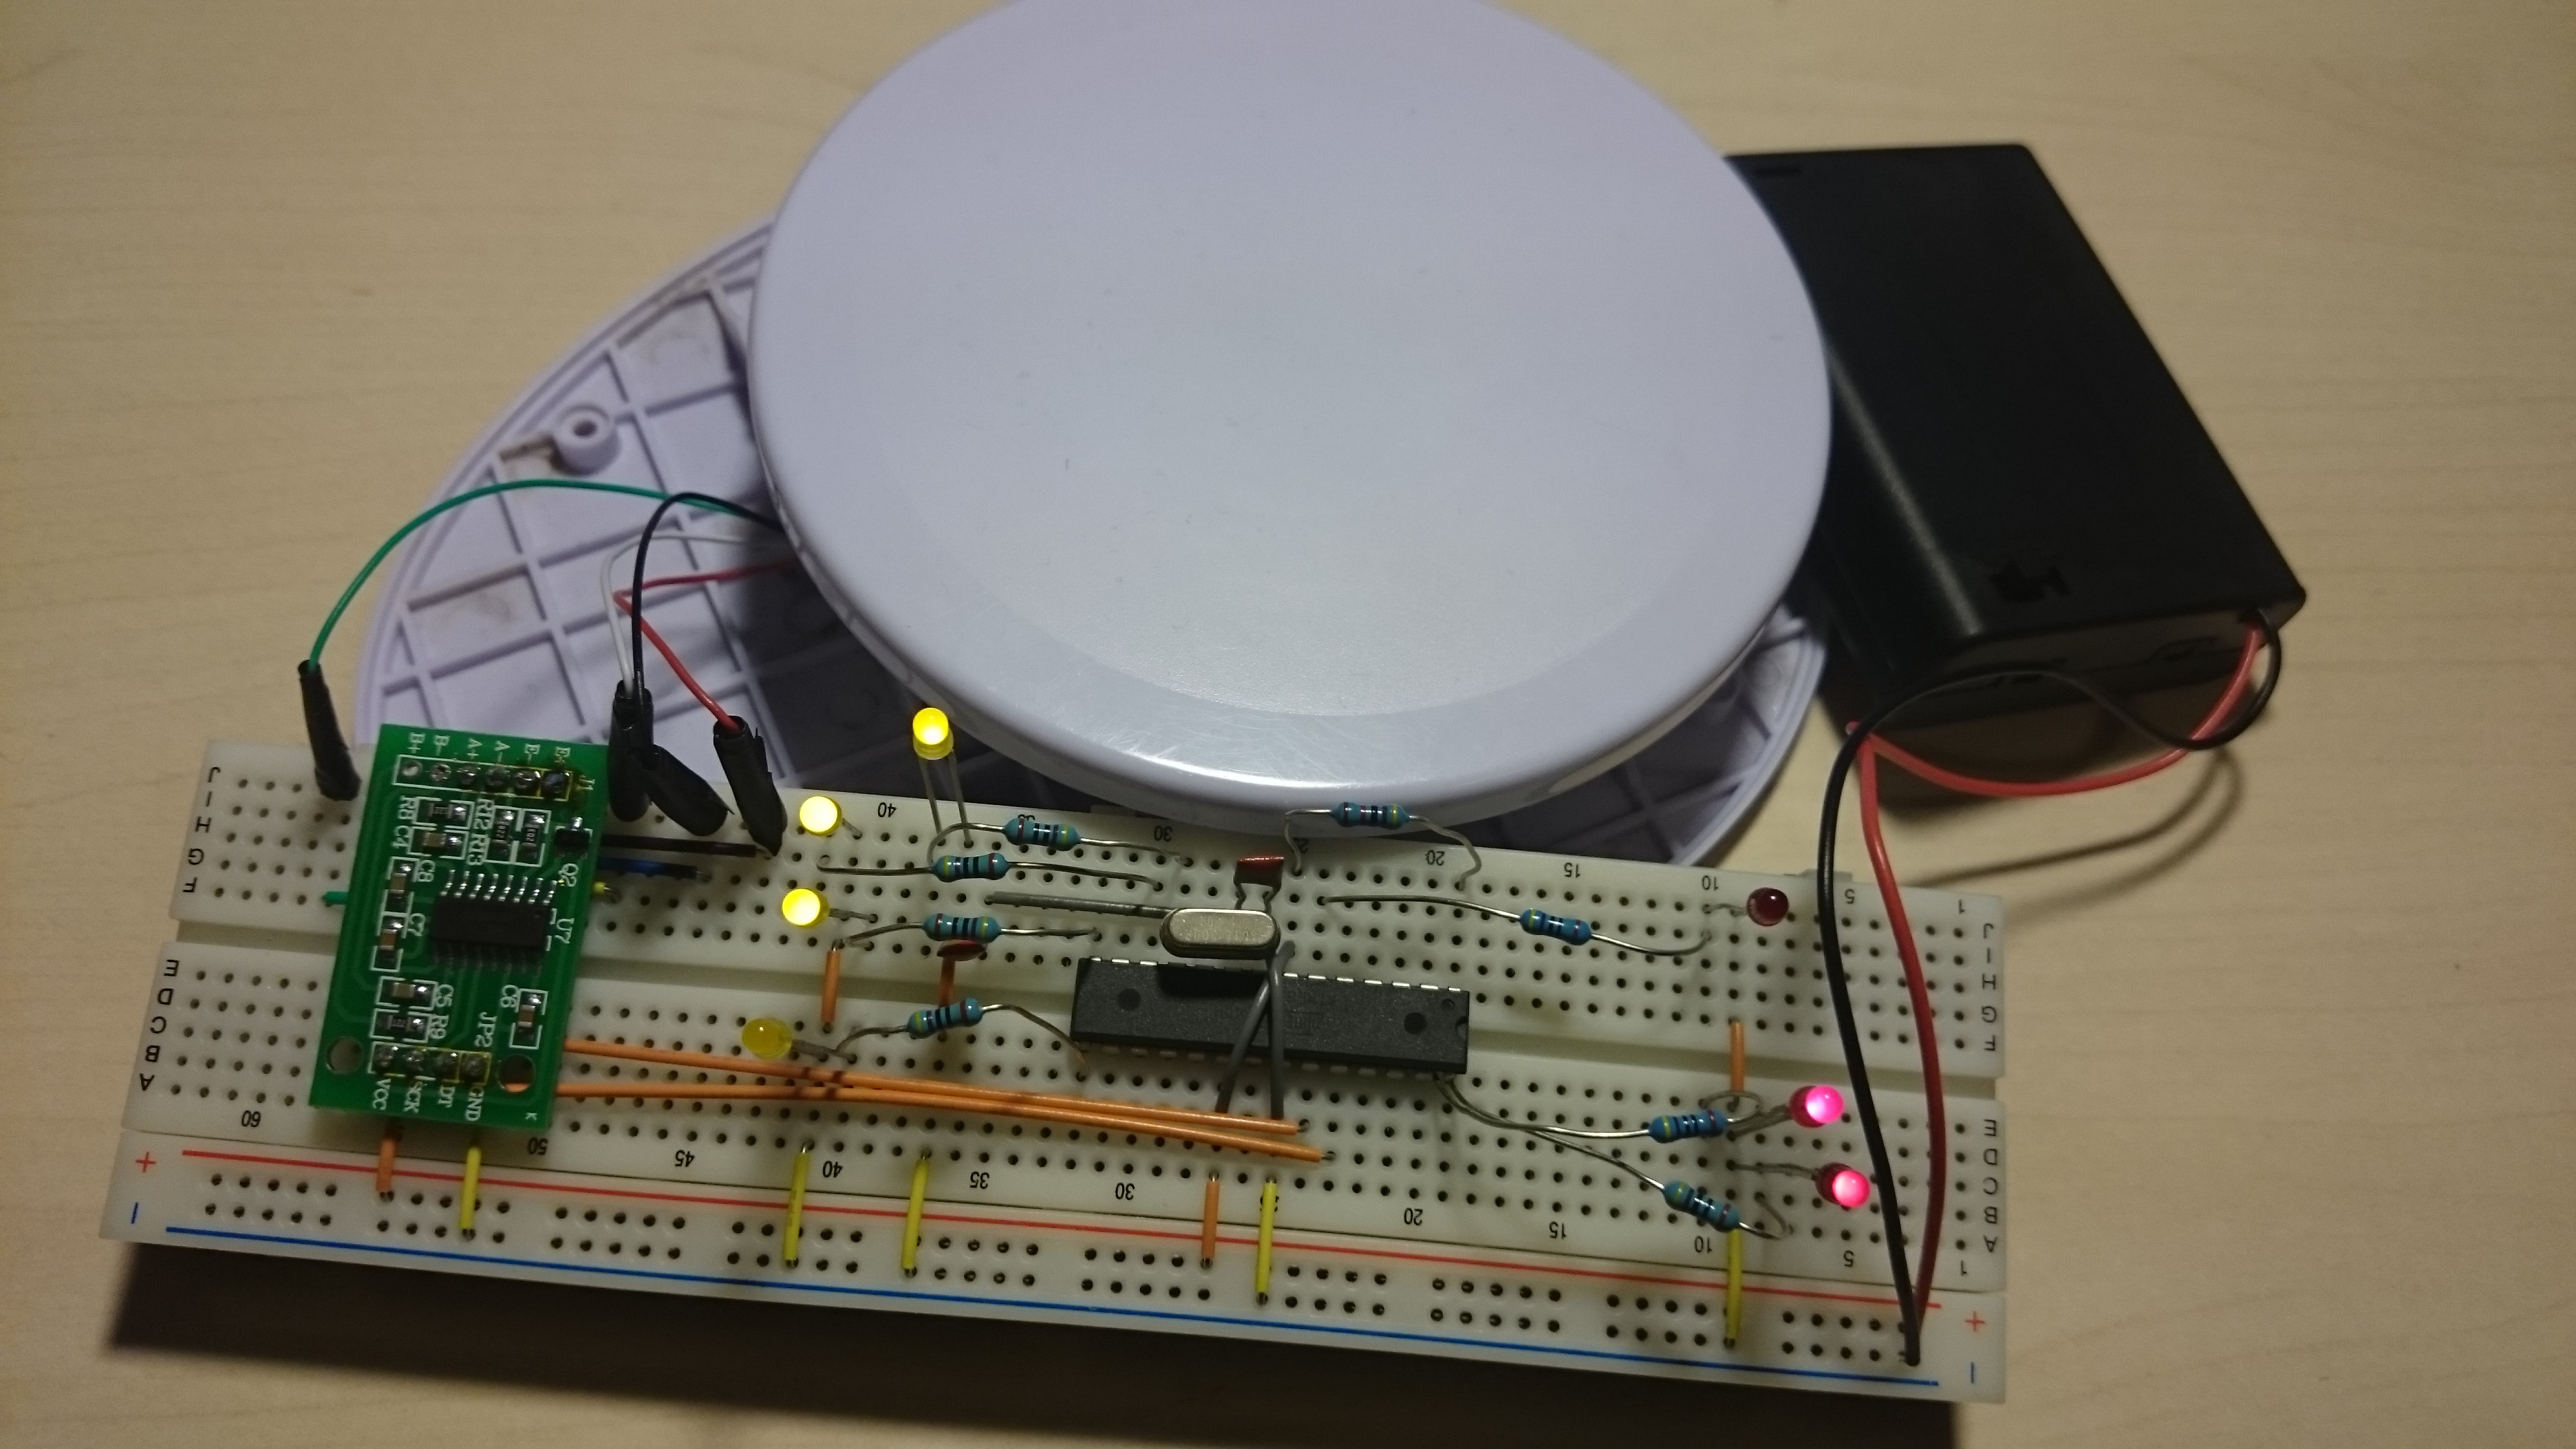
\includegraphics[width=3.5in]{images/prototyp.jpg}
    \caption{Prototyp}
  \label{fig_prototyp}
\end{figure}



%
%\section{Bestandteile}
%
%Unser Bierdeckel besteht aus einer Billigwaage, die die Wägezelle enthält.
%Als Mikrocontroller verwenden wir einen Atmega328p. Da dieser auch auf dem Arduino Uno verbaut
%ist, konnten wir unsere Anwendung zuerst mithilfe des Arduinos auf einem Steckbrett testen.
%Um die Gewichtsdaten, die die Wägezelle liefert verarbeiten zu können verwenden wir den HX711,
%einen 24 Bit Analog zu Digital Konverter für Brückensensoren. Diesen gibt es als fertiges Modul
%zu kaufen (siehe Fig. \ref{fig_HX711_board}). Um anzeigen wie viele neue Biere abgestellt verwenden wir 8 LEDs
%(4 gelbe und 4 rote, mit 3 mm Durchmesser). Damit nicht alle LEDs einzeln an einen Widerstand
%und dann ans Board gelötet werden müssen, haben wir die LEDs in zwei Reihen, mit den
%entsprechenden Anschlüssen und Vorwiderständen, auf eine extra Platine gelötet (siehe Fig. \ref{fig_led_platine}).
%Die Betriebsspannung wird von 3 AA Batterien bereitgestellt. Diese liefern zusammen 4,5 Volt.
%Das ist ausreichend da der Atmega ab 3,7 Volt ein HIGH liest. Die Batterien haben wir in einem
%Batteriefach untergebracht, das schon einen An/Aus Schalter enthält.

% An example of a floating figure using the graphicx package.
% Note that \label must occur AFTER (or within) \caption.
% For figures, \caption should occur after the \includegraphics.
% Note that IEEEtran v1.7 and later has special internal code that
% is designed to preserve the operation of \label within \caption
% even when the captionsoff option is in effect. However, because
% of issues like this, it may be the safest practice to put all your
% \label just after \caption rather than within \caption{}.
%
% Reminder: the "draftcls" or "draftclsnofoot", not "draft", class
% option should be used if it is desired that the figures are to be
% displayed while in draft mode.
%

%\clearpage


\section{Beschaltung des Atmega328p}

%\begin{figure}[!t]
%  \centering
%    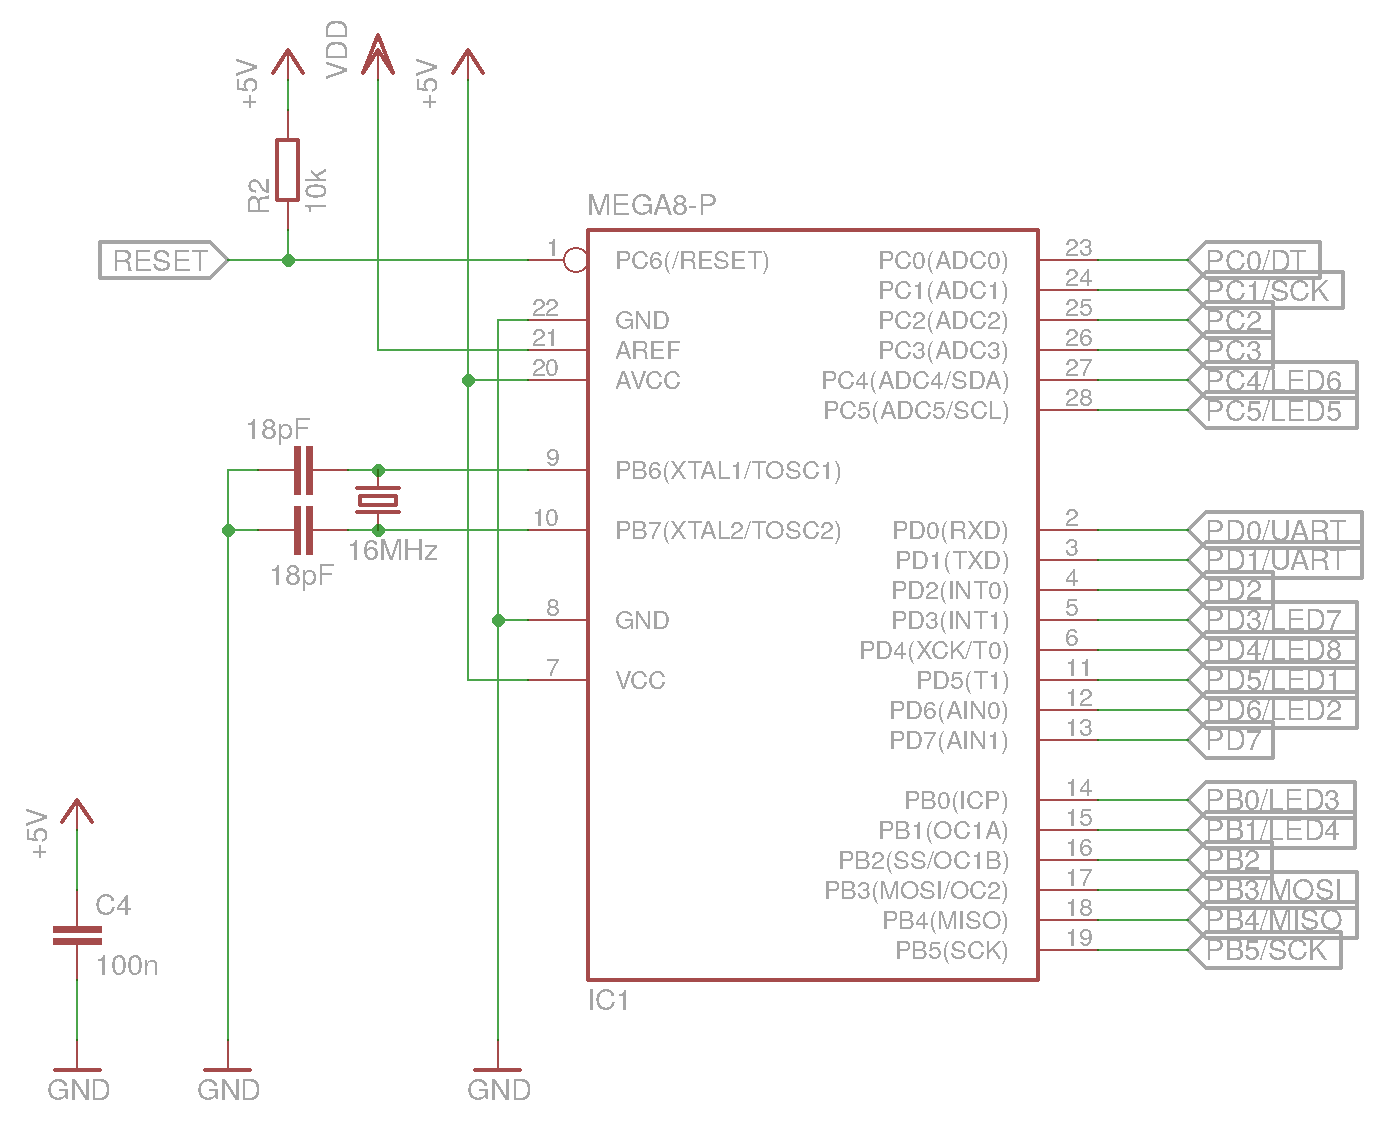
\includegraphics[width=3.5in]{images/atmega328p_pin_belegung.png}
%    \caption{Atmega328p Pin Belegung}
%  \label{fig_atmega328_pin}
%\end{figure}
%
%\begin{figure}[!t]
%  \centering
%    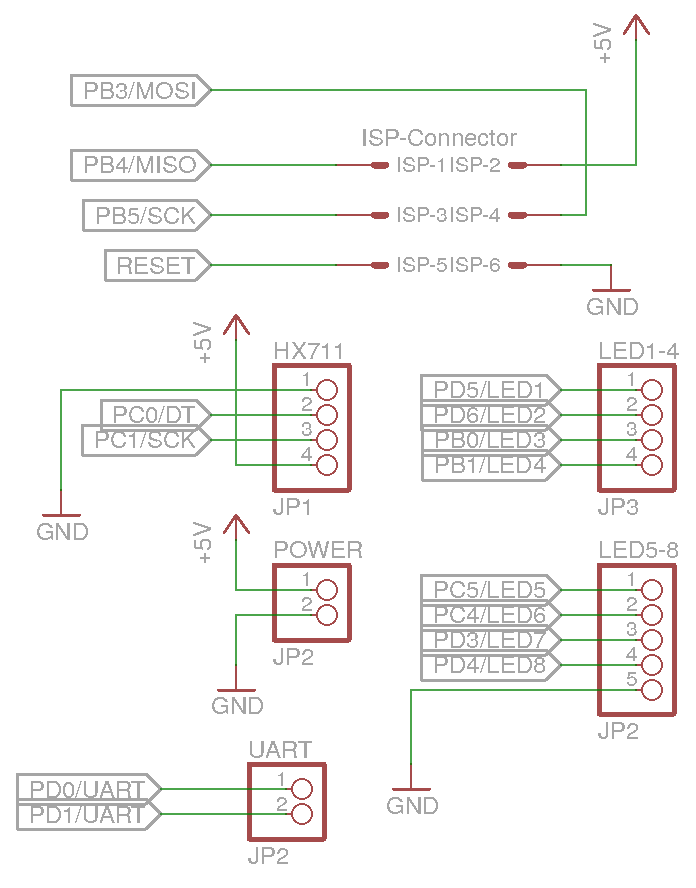
\includegraphics[width=3.5in]{images/bierdeckel_board_connectors.png}
%    \caption{Konnektoren}
%  \label{fig_board_connectors}
%\end{figure}

Um uns das Leben zu erleichtern haben wir eine Platine entworfen, die den Atmega328p enthält
(siehe Fig. \ref{fig_atmega328_pin}). Die anderen Pins sind mit Konnektoren verbunden (siehe Fig. \ref{fig_board_connectors}).
Wir haben also auf dem Board, das den Mikrocontroller enthält mehrere Steckpläzte für die anderen
Komponenten. Das sind also die Steckplätze für:
\begin{itemize}
 \item Das Batteriefach, dass so mit der Platine verbunden wird und die Betriebsspannung (VCC) und die Verbindung zu GND für alle Komponenten liefert.
 \item Den HX711 mit den Pins für VCC, SCK, DT und GND
 \item Die erste Reihe der LEDs auf dem separaten LED Board
 \item Die zweite Reihe der LEDs plus einem Pin für GND
 \item Einen ISP Konnektor
 \item die Stecker für die UART Schnittstelle
\end{itemize}

Die letzten beiden tragen nicht zur Funktion unseres Bierdeckels bei aber wurden eingebaut um den
Bierdeckel neu programmieren (über den ISP Konnektor über die serielle Schnittstelle) zu können
falls man das möchte. Über die UART Schnittstelle kann man das Programm dann debuggen.
Das fertige Layout der Platinen kann man in Fig. \ref{fig_atmega328p_platine} und Fig. \ref {fig_LED_Platine} sehen.


\begin{figure}[htbp]
  \centering
    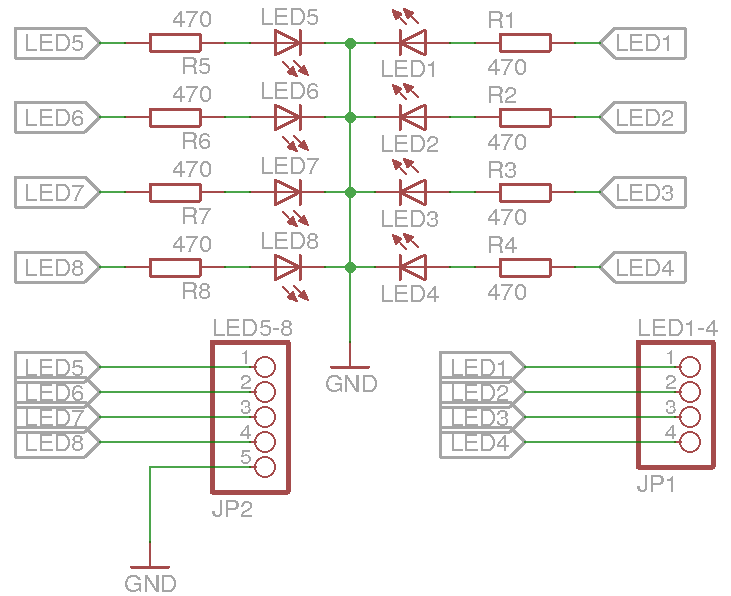
\includegraphics[width=3.5in]{images/LED_Platine_Schema_complete.png}
    \caption{Schema der LED Platine}
  \label{fig_led_platine}
\end{figure}

\begin{figure}[htbp]
  \centering
    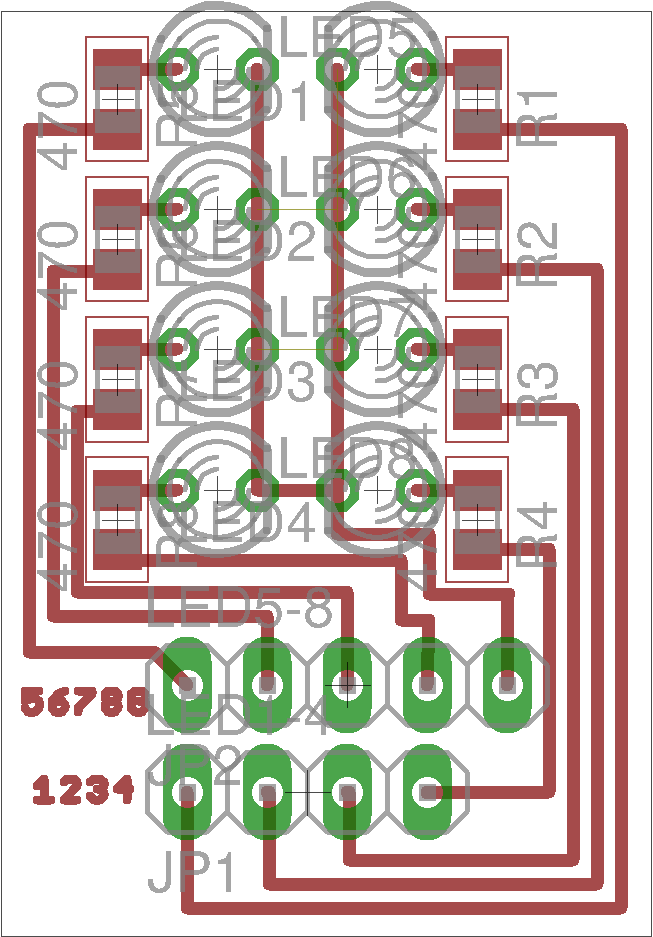
\includegraphics[width=2.7in]{images/LED_Platine.png}
    \caption{Platine mit den Zähler LEDs}
  \label{fig_LED_Platine}
\end{figure}

\begin{figure}[htbp]
  \centering
    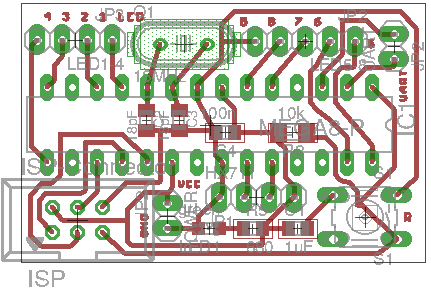
\includegraphics[width=3.5in]{images/atmega328p_platine.png}
    \caption{Platine mit Atmega328p}
  \label{fig_atmega328p_platine}
\end{figure}




%\clearpage
\pagebreak

\section{$\mu$C Programm}
Zur Programmierung des Microcontrollers wurde nach Abbildung \ref{fig_isp} das UNO-Board als ISP genommen.
Hierbei ist jedoch darauf zu achten, RST und GND durch einen zusätzlichen 100$\mu$F Kondensator zu verbinden, um zu verhinden, dass sich der Uno selbst neu programmiert.
\begin{figure}[!h]
  \centering
    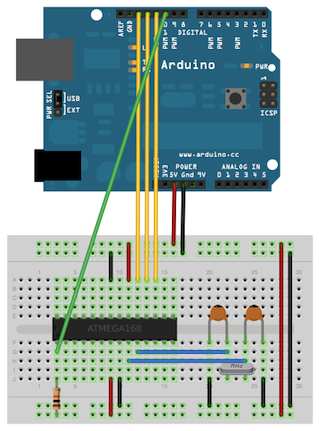
\includegraphics[width=3.5in]{images/isp.png}
    \caption{UNO als ISP}
  \label{fig_isp}
\end{figure}

In folgendem Code wird unser HX711 initialisiert indem wir ihn einmal resetten.
Wir setzen also den Pin PD\_SCK (SCLK im Code) 100$\mu$s lang auf HIGH. Dann lesen wir 32 mal das
Gewicht aus (hx711\_getValue() wird 32 mal aufgerufen) und nehmen den gemittelten Wert als
Offset (entspricht dem Gewicht des leeren Glases,
das zu dem Zeitpunkt auf dem Bierdeckel stehen muss).

\hfil
\lstinputlisting[language=C]{code/hx711_init.c}
\hfil

In hx711\_getValue() wird jetzt gewartet bis DOUT (=SDI im Code) auf LOW wechselt.
Dann werden 24 Taktsignale an PD\_SCK (=SCLK im Code) geschickt um die Daten Bit für Bit auszulesen.
Mit dem 25. Takt wird DOUT wieder auf HIGH gesetzt. Da kein weiterer Takt gesendet wurde,
verwenden wir den Input Kanal A des HX711 mit einem Gain von 128 für das nächste Mal.

\hfil
\lstinputlisting[language=C]{code/hx711_getValue.c}
\hfil

Die Gewichtsdaten liegen jetzt als 24Bit Wert vor. Dieser muss in Gramm umgerechnet werden.
Das geschieht mit einem empirisch bestimmten Skalierungsfaktor.

\hfil
\lstinputlisting[language=C]{code/main.c}
\hfil

In der main() wird nun im Sekundentakt geprüft, ob das abgestellte Glas leer oder voll ist.
hx77\_get\_mg() ruft dabei hx711\_getValue() 32 mal auf um einen gemittelten Wert zu erreichen
und Schwankungen so herauszufiltern. Solange das Glas leer ist blinken die LEDs. Als leer wird das
Glas erkannt, wenn der Inhalt mit einem Gewicht zwischen -50g und 50g gemessen wird.
Als voll wird es erkannt wenn der Inhalt über 480g wiegt.
Wird nun erkannt, dass vom leeren in den vollen Zustand gewechselt wurde, wird daraus geschlossen, dass ein
neues Bier da ist. Dann wird die LED Anzeige eins hochgezählt. Die LEDs werden einzeln über Pins
am Atmega328p angesteuert.
Anschließend geht der Microcontroller für eine Sekunde in den Stromsparmodus.



\section{Verwendung}

Sobald man den Bierdeckel anschaltet, muss das leere Glas auf dem Bierdeckel stehen.
Der HX711 wird dann durch den Atmega initialisiert und es wird das Gewicht des leeren Glases
als Offset errechnet, damit man das Gewicht des Glases nicht mitzählt. Wird nun ein volles Glas
abgestellt, wird erkannt dass vom leeren Zustand in den vollen gewechselt wurde, also ein neues
Bier da ist. Dann wird die LED Anzeige eins hochgezählt. Die Anzeige funktioniert,
wie beim klassischen Bierdeckel, mit den Strich/Zaun Zählsystem. Eine 4er Reihe der LEDs
entspricht also den Strichen und eine den Zäunen. Wenn 4 Strich-LEDs leuchten und eins
hochgezählt wird, dann gehen diese aus und eine weitere Zaun-LED fängt an zu leuchten. 

\section{Ausblick}

Zum aktuellen Stand sind die Einzelteile lose miteinander verbunden. Deswegen ist ein Case
geplant, in dem wir unsere Bestandteile unterbringen wollen. Dieses sollte möglichst klein sein
auch wenn es schwer werden dürfte den Durchmesser und die Höhe eines Standard Bierdeckels einzuhalten.
Auch wäre es wünschenswert von dem ATMega auf einen günstigeren ATTiny umzusteigen, wobei man einen Möglichkeit benötigt meherer LEDs mit weniger Pins anzusteuern.
Denkbare Erweiterungen wären ein Funk Modul (z.B. Bluetooth) einzubauen, über welches der Bedienung signalisiert werden kann, dass das Glas leer ist.
Außerdem wäre es dadurch denkbar eine App zu erstellen, welche es ermöglicht die Kosten anzuzeigen.
Oder auch, nach Eingabe von Körperdaten, zu berechnen ob und wann man wieder fahrtauglich ist.
Eine weitere Erweiterung wäre es Getränke zu unterscheiden, entweder durch direkt Eingabe in der App, oder durch eine Codierung bzw. RFID Chip am Glas.


% references section

% can use a bibliography generated by BibTeX as a .bbl file
% BibTeX documentation can be easily obtained at:
% http://www.ctan.org/tex-archive/biblio/bibtex/contrib/doc/
% The IEEEtran BibTeX style support page is at:
% http://www.michaelshell.org/tex/ieeetran/bibtex/
%\bibliographystyle{IEEEtran}
% argument is your BibTeX string definitions and bibliography database(s)
%\bibliography{IEEEabrv,../bib/paper}
%
% <OR> manually copy in the resultant .bbl file
% set second argument of \begin to the number of references
% (used to reserve space for the reference number labels box)


\begin{thebibliography}{1}

\bibitem{hx711sheet}
AVIA Semiconductor, "24-Bit Analog-to-Digital Converter (ADC) for Weigh Scales", HX711 Datasheet
\\
\bibitem{atmelavrsheet}
Atmel, "ATMEL 8-BIT MICROCONTROLLER WITH 4/8/16/32KBYTES", Datasheet, Nov. 2015
\\
\bibitem{wiki_wheatstone}
https://de.wikipedia.org/wiki/Wheatstonesche\_Messbrücke
\\
\bibitem{tinyusb}
https://github.com/i7sid/diy-tinyusbboard
\\
\bibitem{easylogger}
https://www.obdev.at/products/vusb/easylogger.html


\end{thebibliography}


\end{document}


